\chapter{Introducción}
\label{cap:capitulo1}
\setcounter{page}{1}

\begin{flushright}
\begin{minipage}[]{10cm}
\emph{Quizás algún fragmento de libro inspirador...}\\
\end{minipage}\\

Autor, \textit{Título}\\
\end{flushright}

\vspace{1cm}

El ictus es una enfermedad cerebrovascular (ECV).
El término ictus en latín significa golpe.
Es un trastorno brusco de la circulación cerebral que altera la función de una determinada región del cerebro.

Según la Organización Mundial de la Salud (OMS), es la primera causa de discapacidad y la segunda de muerte en el mundo\footnote{\url{https://www.who.int/srilanka/news/detail/29-10-2022-world-stroke-day-2022}}.
Aproximadamente 15 millones de personas sufren un ictus cada año; entre ellas, 5 millones mueren y otros 5 millones quedan con alguna discapacidad permanente, lo que supone una carga significativa para las familias y comunidades\footnote{\url{https://www.emro.who.int/health-topics/stroke-cerebrovascular-accident/index.html}}.

Según el Sistema Nacional de Salud, \cite{perales1a}, cada año, alrededor de $120.000$ personas sufren un ictus en España.
La edad es uno de los factores de riesgo principales de esta enfermedad, aunque ocurre en todos los grupos de edad.
En los últimos años la incidencia en adultos jóvenes ha aumentado un $40\%$.
Los mejores sistemas de diagnóstico, así como el aumento de consumo de drogas, pueden ser algunas de las causas de este aumento.
Se estima que 1 de cada 4 personas en el mundo sufrirán un ictus a lo largo de su vida.
Gracias a los avances científicos, tecnológicos y clínicos se han podido desarrollar tratamientos para minimizar los déficits que produce.
En la Imagen \ref{fig:grafica}, se muestra la prevalencia registrada de enfermedad cerebrovascular por 1.000 habitantes, según sexo y edad en España en 2019.\\

\begin{figure}[ht!]
	\centering
	\begin{minipage}{0.95\linewidth}
		\centering
		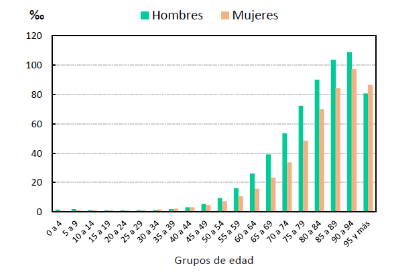
\includegraphics[width=\linewidth]{figs/edad_ictus_es.png}
	\end{minipage}
	\caption[Prevalencia registrada de enfermedad cerebrovascular según sexo y edad en España, 2019]{Prevalencia registrada de enfermedad cerebrovascular según sexo y edad en España, 2019}
	\label{fig:grafica}
\end{figure}

Según la OMS, la rehabilitación se define como un $"$conjunto de medidas que ayudan a las personas que tienen o probablemente tendrán una discapacidad, a conseguir y mantener el funcionamiento óptimo en interacción con su ambiente".

Asimismo el Grupo de Estudio de ECV de la Sociedad Española de Neurología (SEN), considera que la rehabilitación es una de las partes más importantes para el tratamiento de la mayoría de los pacientes que han sufrido un ictus y han sobrevivido.
Suele comenzarse en los primeros días de estancia en el hospital y se recomienda a cualquier paciente que, previo al ictus, fuese autosuficiente.
Es importante entender que es difícil volver a una situación igual a la inicial.
El objetivo fundamental es ayudar al paciente a adaptarse, ya que el ictus se recupera de forma espontánea o puede no recuperarse nunca, dependiendo de su gravedad, la cual determina la duración del programa de rehabilitación y su intensidad.
Los seis primeros meses son los de mayor importancia para recuperar los movimientos voluntarios.
Con un programa adecuado, un $1/3$ de los pacientes vuelven a su trabajo\footnote{\url{http://ictus.sen.es}}.

El plan de acción europeo para el ictus 2018-2030, propuesto por la Alianza Europea contra el ictus \cite{perales2a}, surge con el objtivo de mejorar el cuidado de los ictus y la vida después de estos.
Entre los objetivos generales para el año 2030 se encuentran:
\begin{enumerate}
    \item Garantizar que al menos el $90\%$ de la población tenga acceso a la rehabilitación precoz en la unidad de ictus.
    \item Proporcionar el alta precoz con apoyo a por lo menos el $20\%$ de los pacientes de ictus en todos los países.
    \item Ofrecer programas de acondicionamiento físico a todos los pacientes de ictus que viven en la comunidad.
    \item Proporcionar un plan documentado para la rehabilitación en la comunidad y el apoyo al autocontrol de todos los pacientes de ictus con dificultades residuales al recibir el alta hospitalaria.
    \item Garanticen que se revisan las necesidades de rehabilitación, y otras, de todos los pacientes de ictus entre los 3 y 6 meses después de sufrirlo y anualmente a partir de ese momento.
\end{enumerate}\

Según la Socidad Española de Rehabilitación y Medicina Física (SERMEF), el $50\%$ de los supervivientes de ictus sufre secuelas y la rehabilitación temprana reducirá su dependencia en un $20\%$.
Además, manifiesta que existen desigualdades en los accesos a estos tratamientos entre Comunidades Autónomas.
Entre las principales secuelas se encuentra la pérdida de función motora, que afecta entre el $50\%$ y $85\%$ de los pacientes, trastornos del habla, disfunciones cognitivas, eplasticidad y debilidad muscular\footnote{\url{https://www.sermef.es/el-50-de-los-supervivientes-de-ictus-sufre-secuelas-y-la-rehabilitacion-temprana-reducira-su-dependencia-en-un-20/}}.\\

Una vez conocida la prevalencia del ictus y la importancia de la rehabilitación, se valoran las ventajas de introducir la robótica en este campo.

En el artículo de \cite{perales3a}, se analizaban los beneficios de la rehabilitación asistida por robots frente a la fisioterapia tradicional.
Esta consiste en la realización de ejercicios manuales por parte de un fisioterapeuta cualificado, aunque son muy exigentes en cuanto al tiempo de dedicación al paciente.
Por ello se comenzó una investigación para utilizar dispositivos mecánicos en el proceso de rehabilitación.

Varios autores han propuesto el uso de dispositivos robóticos para la rehabilitación del miembro superior.
Existen diversos modelos como el robot MIT-MANUS o Gentle/s.
El primero, fue desarrollado por los investigadores \cite{perales3b}, Volpe y Hogan, del Massachusetts Institute of Technology y del Burke Medical Research Institute.
Se ha demostrado que reduce de manera eficaz el tiempo de recuperación motriz del paciente al realizar los ejercicios apropiados para la rehabilitación del hombro y el codo.
El segundo, es un robot de asistencia robótica en rehabilitación neurológica y motora.
Como se indica en el artículo \cite{perales3c}, la tasa de recuperación fue mayor durante la fase de terapia mediada por el robot que en la fase base para la mayoría de los sujetos.
Según \cite{perales3d}, la rehabilitación asistida por robot ofrece ventajas importantes respecto a la fuerza muscular, el aumento de las puntuaciones clínicas y un grado mayor de recuperación de la independencia funcional.
En las Imagenes \ref{fig:mitmanus} y \ref{fig:gentles} se pueden observar los primeros robots que se deserrollaron para la rehabilitación en pacientes post-ictus.

\begin{figure}[ht!]
	\centering
	\begin{minipage}{0.55\linewidth}
		\centering
		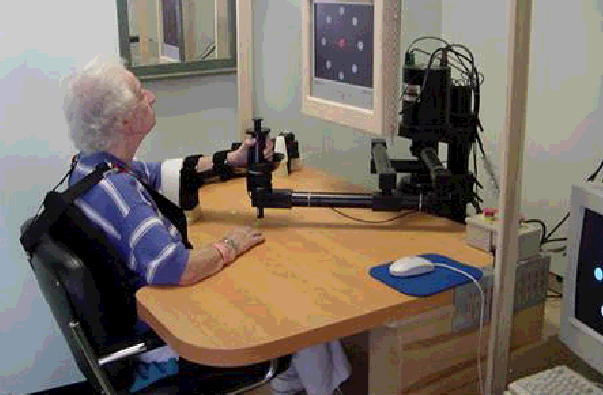
\includegraphics[width=\linewidth]{figs/mit_manus.png}
	\end{minipage}
	\caption[MIT-MANUS (Interactive Motion Technologies Cambridge)]{MIT-MANUS (Interactive Motion Technologies Cambridge)}
	\label{fig:mitmanus}

	\centering
	\begin{minipage}{0.55\linewidth}
		\centering
		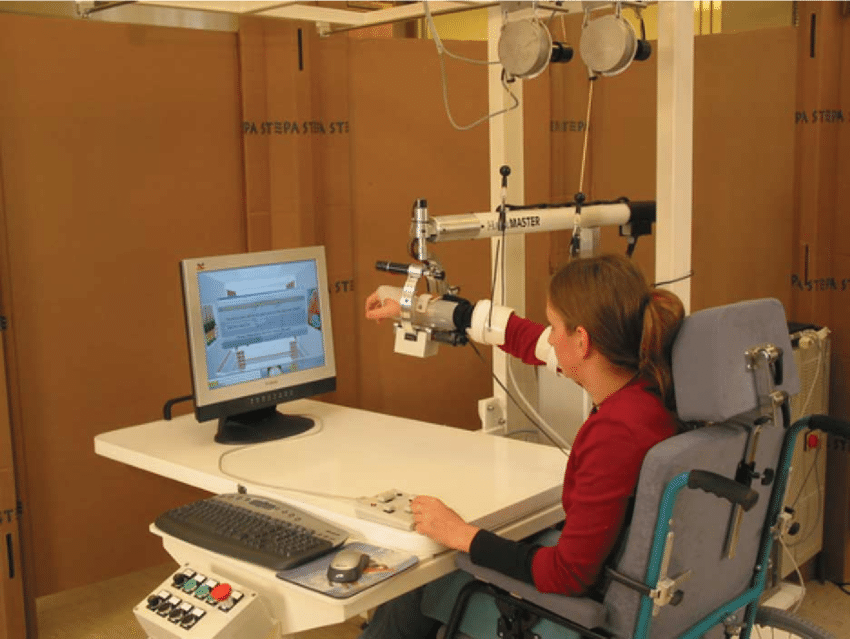
\includegraphics[width=\linewidth]{figs/gentles.png}
	\end{minipage}
	\caption[Prototipo comercial Gentle/s para neurorrehabilitación mediada por máquinas]{Prototipo comercial Gentle/s para neurorrehabilitación mediada por máquinas}
	\label{fig:gentles}
\end{figure}

En los últimos $5$ años, se han realizado distintos análisis sobre la efectividad de la incorporación robótica en la rehabilitación.

\begin{itemize}
	\item En el artículo \cite{perales4a} se realiza un metanálisis para medir el rendimiento de las extremidades superiores de $18$ estudios. Concluyó que la rehabilitación con brazo robótico y una duración de entre $30$ y $60$ minutos por sesión, mejoraron significativamente la función de las extremidades superiores.
	\item En el artículo \cite{perales4b} se indica que la terapia con robots es una terapia relativamente nueva, permite aumentar el número de repeticiones en la ejecución de movimientos específicos y concluyen que presenta beneficios en todas las fases de rehabilitación del ictus.
	\item En el artículo \cite{perales4c} se realiza una búsqueda para analizar el efecto de los robots de rehabilitación seleccionando $18$ ensayos con $573$ pacientes con ictus y los resultados mostraron que los pacientes que reciben este tio de terapia mejoraron significativamente las puntaciones de evaluación motora. Concluyeron que el entrenamiento asistido por robot es superior al entrenamiento convencional, lo que respalda el uso de robots en la práctica clínica.
\end{itemize}\

Para que la rehabilitación del paciente no resulte monótona y desmotivadora, es interesante inluir entornos gamificados en las terapias.
Con ello se consigue un mejor compromiso y adherencia, un incremento de la motivación del paciente y permite la personalización del ejercicio.
La gamificación permite evaluar el progreso del paciente mediante distintas mecánicas como desafíos y recompensas.
